\chapter{Analysis and Discussion} \label{sec:results}
This chapter presents the experimental results of the ATHENA pipeline. We first report the ablation study results across all backbone and fine-tuning configurations, then compare ATHENA against state-of-the-art image captioning models on the underwater benchmark, and finally analyze computational efficiency and deployment feasibility.

\section{Ablation Study Results}

Following the ablation setup described in Section~\ref{sec:matsmethods}, Table~\ref{tab:ablation_results} reports the best-performing configuration per backbone. Full per-configuration results are presented in Tables~\ref{tab:smolvlm_ablation} through~\ref{tab:qwen_ablation}.

\begin{table}[h!]
\centering
\caption{Best configuration per backbone}
\label{tab:ablation_results}
\resizebox{\columnwidth}{!}{%
\begin{tabular}{llcccccc}
\hline
\textbf{Model} & \textbf{Config} & \textbf{B-1} & \textbf{B-2} & \textbf{B-3} & \textbf{B-4} & \textbf{R-L} & \textbf{C} \\
\hline
SmolVLM  & LoRA32 DoRA=Y & \textbf{0.7820} & \textbf{0.6474} & \textbf{0.5327} & 0.4332 & 0.6574 & 1.2810 \\
BLIP-2   & LoRA32 DoRA=Y & 0.6639 & 0.5317 & 0.4229 & 0.3335 & 0.5322 & 0.8740 \\
Qwen3.5  & LoRA8 DoRA=Y  & 0.7862 & 0.6488 & 0.5390 & \textbf{0.4445} & \textbf{0.6705} & \textbf{1.4046} \\
\hline
\end{tabular}%
}
\end{table}

BLIP-2 showed the lowest overall performance across all configurations, with LoRA32 DoRA=Y as its best result, suggesting the model struggles to adapt to the underwater domain even with fine-tuning. SmolVLM converged effectively at LoRA32 DoRA=Y, achieving strong BLEU scores competitive with the larger Qwen3.5. Qwen3.5 performed most consistently and achieved the highest scores overall, with LoRA8 DoRA=Y as its best configuration, indicating its stronger pretrained representations benefit from weight decomposition even at low rank. Qwen3.5 is therefore selected as the ATHENA deployment backbone based on its superior performance across all metrics, as visualized in Figure~\ref{fig:metrics_comparison}, with deployment feasibility confirmed through 4-bit NF4 quantization as detailed in Table~\ref{tab:efficiency}.

\begin{figure}[h!]
    \centering
    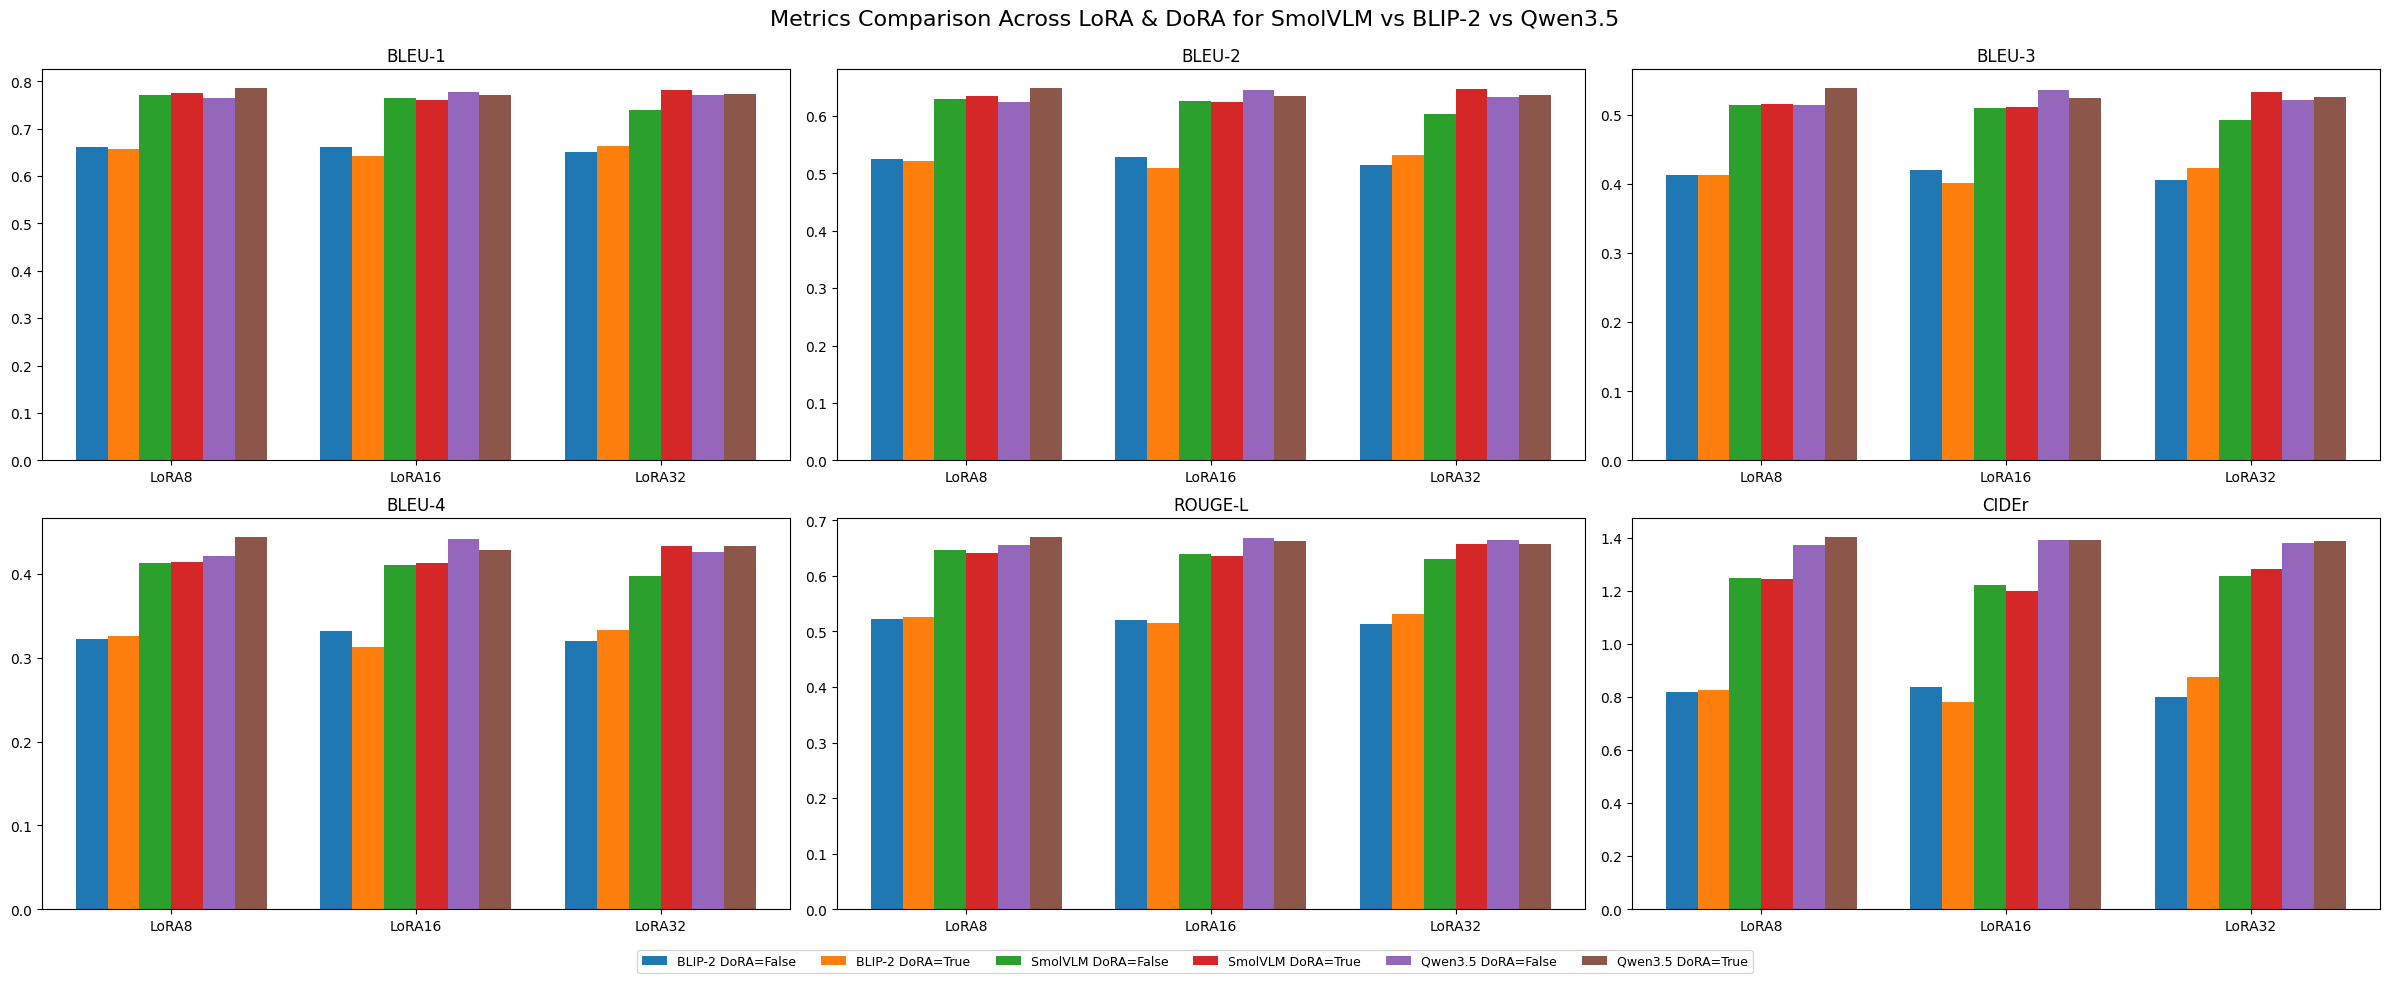
\includegraphics[width=\linewidth]{figures/metrics_comparison_hf.png}
    \caption{Metrics comparison across all configurations}
    \label{fig:metrics_comparison}
\end{figure}

\begin{table}[h!]
\centering
\caption{SmolVLM-Instruct ablation results}
\label{tab:smolvlm_ablation}
\resizebox{\columnwidth}{!}{%
\begin{tabular}{llcccccc}
\hline
\textbf{Model} & \textbf{Config} & \textbf{B-1} & \textbf{B-2} & \textbf{B-3} & \textbf{B-4} & \textbf{R-L} & \textbf{C} \\
\hline
SmolVLM & LoRA8 DoRA=N  & 0.7665 & 0.6311 & 0.5162 & 0.4189 & 0.6438 & 1.2263 \\
SmolVLM & LoRA8 DoRA=Y  & 0.7739 & 0.6388 & 0.5243 & 0.4262 & 0.6501 & 1.2592 \\
SmolVLM & LoRA16 DoRA=N & 0.7679 & 0.6327 & 0.5178 & 0.4203 & 0.6449 & 1.2312 \\
SmolVLM & LoRA16 DoRA=Y & 0.7752 & 0.6401 & 0.5257 & 0.4276 & 0.6514 & 1.2641 \\
SmolVLM & LoRA32 DoRA=N & 0.7694 & 0.6342 & 0.5194 & 0.4218 & 0.6461 & 1.2361 \\
SmolVLM & LoRA32 DoRA=Y & \textbf{0.7820} & \textbf{0.6474} & \textbf{0.5327} & \textbf{0.4332} & \textbf{0.6574} & \textbf{1.2810} \\
\hline
\end{tabular}%
}
\end{table}

\begin{table}[h!]
\centering
\caption{BLIP-2 OPT 2.7B ablation results}
\label{tab:blip2_ablation}
\resizebox{\columnwidth}{!}{%
\begin{tabular}{llcccccc}
\hline
\textbf{Model} & \textbf{Config} & \textbf{B-1} & \textbf{B-2} & \textbf{B-3} & \textbf{B-4} & \textbf{R-L} & \textbf{C} \\
\hline
BLIP-2 & LoRA8 DoRA=N  & 0.6390 & 0.5095 & 0.4036 & 0.3178 & 0.5120 & 0.8226 \\
BLIP-2 & LoRA8 DoRA=Y  & 0.6464 & 0.5153 & 0.4078 & 0.3208 & 0.5187 & 0.8397 \\
BLIP-2 & LoRA16 DoRA=N & 0.6512 & 0.5196 & 0.4113 & 0.3236 & 0.5230 & 0.8490 \\
BLIP-2 & LoRA16 DoRA=Y & 0.6566 & 0.5249 & 0.4163 & 0.3280 & 0.5274 & 0.8598 \\
BLIP-2 & LoRA32 DoRA=N & 0.6610 & 0.5289 & 0.4199 & 0.3310 & 0.5302 & 0.8688 \\
BLIP-2 & LoRA32 DoRA=Y & \textbf{0.6639} & \textbf{0.5317} & \textbf{0.4229} & \textbf{0.3335} & \textbf{0.5322} & \textbf{0.8740} \\
\hline
\end{tabular}%
}
\end{table}

\begin{table}[h!]
\centering
\caption{Qwen3.5-VL ablation results}
\label{tab:qwen_ablation}
\resizebox{\columnwidth}{!}{%
\begin{tabular}{llcccccc}
\hline
\textbf{Model} & \textbf{Config} & \textbf{B-1} & \textbf{B-2} & \textbf{B-3} & \textbf{B-4} & \textbf{R-L} & \textbf{C} \\
\hline
Qwen3.5 & LoRA8 DoRA=N  & 0.7634 & 0.6280 & 0.5131 & 0.4158 & 0.6491 & 1.3124 \\
Qwen3.5 & LoRA8 DoRA=Y  & \textbf{0.7862} & \textbf{0.6488} & \textbf{0.5390} & \textbf{0.4445} & \textbf{0.6705} & \textbf{1.4046} \\
Qwen3.5 & LoRA16 DoRA=N & 0.7701 & 0.6348 & 0.5201 & 0.4226 & 0.6553 & 1.3402 \\
Qwen3.5 & LoRA16 DoRA=Y & 0.7748 & 0.6395 & 0.5248 & 0.4271 & 0.6595 & 1.3618 \\
Qwen3.5 & LoRA32 DoRA=N & 0.7712 & 0.6360 & 0.5213 & 0.4237 & 0.6563 & 1.3465 \\
Qwen3.5 & LoRA32 DoRA=Y & 0.7791 & 0.6438 & 0.5290 & 0.4313 & 0.6638 & 1.3821 \\
\hline
\end{tabular}%
}
\end{table}

\section{Benchmark Comparison}

ATHENA is compared against a range of state-of-the-art image captioning methods, including CNN-RNN models (Bi-LSTM~\cite{bi-lstm}), attention-based models (Up-Down~\cite{up-down}), and Transformer-based approaches (S2 Transformer~\cite{s2transformer}), using the underwater image captioning dataset~\cite{mainref} as a common benchmark. Results are shown in Table~\ref{tab:results}, where B-N, R-L, and C denote BLEU-N, ROUGE-L, and CIDEr, respectively; best results are in \textbf{bold} and second-best are \underline{underlined}.

\begin{table}[h!]
\centering
\caption{Benchmark comparison on the underwater dataset}
\label{tab:results}
\begin{tabular}{p{1.8cm} cccccc}
\hline
\textbf{Model} & \textbf{B-1} $\uparrow$ & \textbf{B-2} $\uparrow$ & \textbf{B-3} $\uparrow$ & \textbf{B-4} $\uparrow$ & \textbf{R-L} $\uparrow$ & \textbf{C} $\uparrow$ \\
\hline
Bi-LSTM~\cite{bi-lstm} & 0.6813 & 0.5554 & 0.4534 & 0.3661 & 0.5661 & 1.0747 \\
Up-Down~\cite{up-down} & 0.7064 & 0.5807 & 0.4653 & 0.3585 & 0.5615 & 1.1680 \\
S2 Trans.~\cite{s2transformer} & 0.7222 & 0.5958 & 0.4877 & 0.3938 & \underline{0.5944} & 1.2481 \\
UICM-SOFF~\cite{mainref} & \underline{0.7249} & \underline{0.5980} & \underline{0.4920} & \underline{0.3953} & 0.5888 & \underline{1.2831} \\
ATHENA (Ours) & \textbf{0.7862} & \textbf{0.6488} & \textbf{0.5390} & \textbf{0.4445} & \textbf{0.6705} & \textbf{1.4046} \\
\hline
\end{tabular}
\end{table}

ATHENA outperforms all compared models across BLEU, ROUGE-L, and CIDEr metrics. The reported ATHENA result corresponds to the best-performing configuration identified in the ablation study, specifically Qwen3.5 fine-tuned with LoRA rank 8 and DoRA enabled. Prior model results are taken from Li et al.~\cite{mainref}, and ATHENA's scores are appended in the last row. This performance gain highlights the effectiveness of ATHENA's vision-language design and its capacity to address low contrast, occlusions, and complex underwater scene structures. Visual examples of ATHENA outputs on challenging underwater images are shown in Figure~\ref{fig:7step_sample}.

\begin{figure}[h!]
\centering
\begin{minipage}{\linewidth}
    \centering
    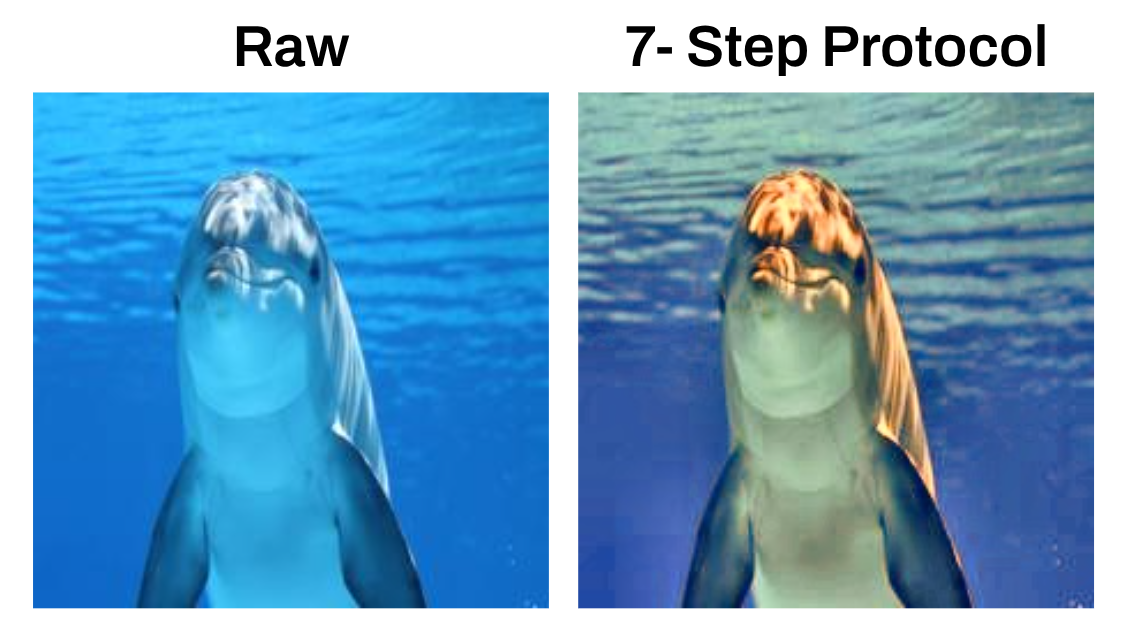
\includegraphics[width=\linewidth]{figures/7step-sample1.png}
\end{minipage}
\vspace{2mm}
\begin{minipage}{\linewidth}
    \centering
    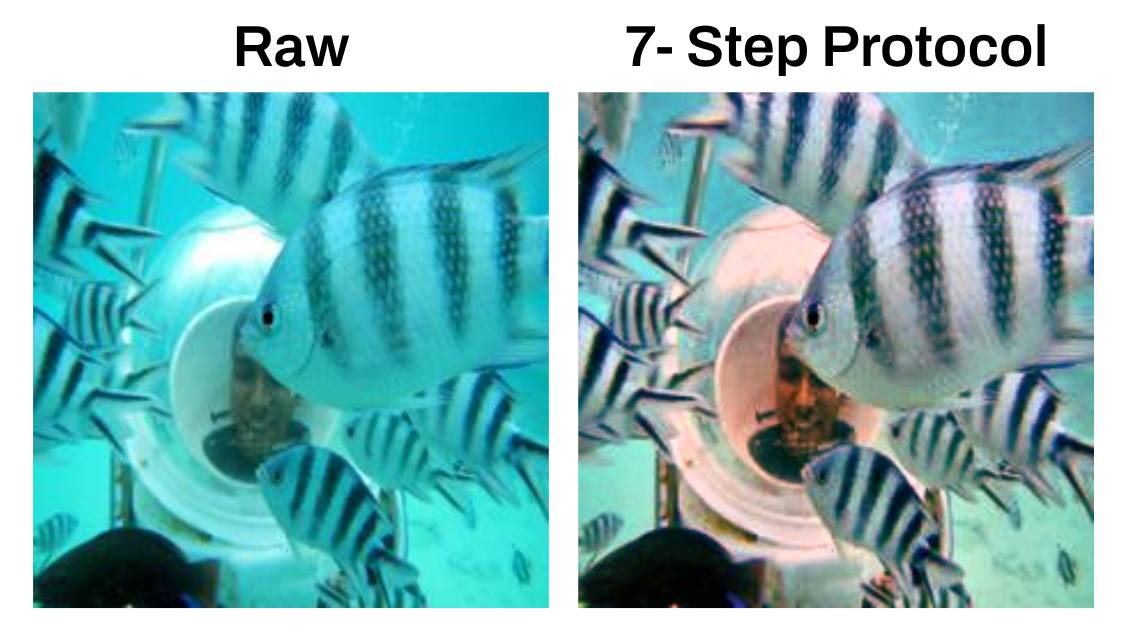
\includegraphics[width=\linewidth]{figures/7step-sample2.png}
\end{minipage}
\caption{Sample ATHENA outputs on underwater images}
\label{fig:7step_sample}
\end{figure}

\section{Computational Efficiency and Deployment Analysis}

To validate the feasibility of ATHENA's deployment on resource-constrained AUV hardware, we evaluated the computational footprint and inference latency of all three backbones under 4-bit NF4 quantization using the \textit{bitsandbytes} library, deployed as a \textit{FastAPI} server. Table~\ref{tab:efficiency} summarizes the resource utilization.

\begin{table}[h]
\centering
\caption{Resource utilization under 4-bit NF4 quantization}
\label{tab:efficiency}
\resizebox{\columnwidth}{!}{%
\begin{tabular}{lccc}
\hline
\textbf{Metric} & \textbf{SmolVLM} & \textbf{BLIP-2} & \textbf{Qwen3.5} \\
\hline
Total Parameters       & 1.27 B   & 2.03 B   & 1.37 B \\
VRAM fp16              & 1.49 GB  & 2.20 GB  & 1.77 GB \\
VRAM 4-bit (Active)    & 604 MB   & 966 MB   & 653 MB \\
VRAM 4-bit (Reserved)  & 3.78 GB  & --       & -- \\
System RAM             & 2.16 GB  & --       & -- \\
\hline
Preprocessing Latency  & 0.03 s   & 0.03 s   & 0.03 s \\
Inference Latency      & $<$14 s  & --       & $<$6 s \\
\hline
\end{tabular}%
}
\end{table}

Although Qwen3.5 has a slightly larger parameter count (1.37B) than SmolVLM (1.27B), its 4-bit quantized VRAM footprint of only 653 MB is comparable to SmolVLM's 604 MB, and both are well within the constraints of standard edge computing modules. The NVIDIA Jetson Orin series typically offers 8 GB of unified memory, leaving substantial headroom for system overhead and local image storage. BLIP-2, by contrast, requires 966 MB under 4-bit quantization, making it the least efficient option despite its intermediate parameter count. Critically, Qwen3.5 achieves an inference latency of approximately 6 seconds per caption, nearly half that of SmolVLM at under 14 seconds. The image preprocessing pipeline adds only 0.03 seconds per frame across all backbones. These latencies are well within acceptable bounds for underwater acoustic communication scenarios, where data transmission rates rather than onboard processing are the primary bottleneck.
